In order to calculate the transport of electrons in NPG one must obtain the Green's functions and self energies related to the unit cells of the system. In order to do so, a recursion algorithm must be implemented as calculations become too costly for the system, even if it is small. Especially the inversion of matrices required to obtain the Green's function can be very demanding computationally, when the system contains a lot of atoms. The recursion algorithm reduces the size of the system and thereby the amount of computational time required to obtain both the first cell Green's function, the Green's function within the chain (of repeated unit cells) sometimes called \(\mathbf{G}_{bulk}\) as well as the self energies related to those Green's functions. The recursion works by utilising that one can remove every second cell in an infinite chain of cells. As the chain originally was infinite, removing every second cell will just yield a new infinite chain. Every cell has with it, its hopping matrices and hamiltonian. The removal of every second cell is iterated, changing the effective interaction between the cells and thus the hopping matrices as well as the hamiltonians of the system. In the end the recursion algorithm produces re-normalised hamiltonians and hopping matrices, which can be used to obtain the Green's functions and self energies. 
\subsection{Obtaining first cell self energy and Green's function}\label{recursionroutinesec}
For simplicity and in order to check whether the routine would yield the results expected, the starting point is a simple system containing only 4 atoms in the unit cell. The idea is to make a function that takes in an energy, a hamiltonian (alternatively two in case there is a special site in the molecule) and a hopping matrix as arguments and outputs the Green's function at the zeroth site as well as the self energies going left and right. Firstly all the necessary variables are defined. The first of these consists of a complex number matrix which has the value \(E + i\eta\) in the diagonal and dimension identical to that of the hamiltonian given as argument. Here \(E\) is the energy which the function takes as an argument and \(\eta\) is a small number (in specific case \(1\times10^{-6}\)). Note that \(\eta\) should not be made too small as it will yield incorrect results. The rest of the variables are the hamiltonian, hopping matrices and Green's functions. They are defined as: \(a0 = V^{\dagger}, \ b0 = V, \ e0_{s} = h, \ e_{0} = h, \ g0 = (z-e0)^{-1}\). Note that the hamiltonian \(h\) here is the same for both \(e0_{s}\) and \(e0\) as the zeroth cell is identical to those of the rest of the molecule. Now that the variables is defined, the actual recursion can begin. As the recursion is an algorithm that runs for an arbitrary amount of iterations, a while loop is chosen to run the iterations until a threshold has been reached. The threshold is defined as the absolute maximum value in the hopping matrix \(a0\) approaches zero. In this specific case it was set to \(1\times10^{-8} \). Within this while loop a range matrix multiplications are computed. These constitutes the actual recursion and their order are of big importance for a correct result. Following is a list of these matrix multiplications: 
\begin{align*}
a1 &= a0\ g0\ a0\\
b1 &= b0\ g0\ b0\\
e1 &= e0 + a0\ g0\ b0 + b0\ g0\ a0 \\
e1_{s} &= e0_{s} + a0\ g0\ b0 \\
g1 &= (z - e1)^{-1}
\end{align*}
As stated above in the equations, the matrix product are defined as new variables with a \(+1\) variable name. This is all very well but the while loop would stop here because of the definition of new variables. It is therefore necessary to redefine the new variables in terms of the old ones (f.ex. \(a0 = a1\)) an as such the while loop will continue until the threshold has been reached. For the rest of the function the only thing left to do is to define the self energies and the first cell Green's function using the variables obtained from the while loop. These are simply given as: 
\begin{align*}
    \mathbf{\Sigma}_R &= e_s - h \\
    \mathbf{\Sigma}_L &= e - h - \mathbf{\Sigma}_R \\
    \mathbf{G00} &= (z - e_s)^{-1}
\end{align*}
Where \(e_s\) and \(e\) are the resulting matrices from the while loop. The first cell Green's function as well as the self energies has now been obtained by recursion. 
\subsection{Plotting the real and imaginary part of the first cell Green's function}
As a good way to check whether the recursion routine has been implemented successfully, the real and imaginary part of the Green's function can be plotted with a relatively simple approach including a for loop:
The imaginary part of the Green's function is especially important as it represents the local density of states LDOS. Following is the plot of the real and imaginary part of the first cell Green's function obtained by the recursion routine for the simple four atom unit cell described in \cref{recursionroutinesec}. In \cref{imrealplot} a plot of the imaginary and real part of the resulting Green's function can be seen. 
\begin{figure}
    \centering
    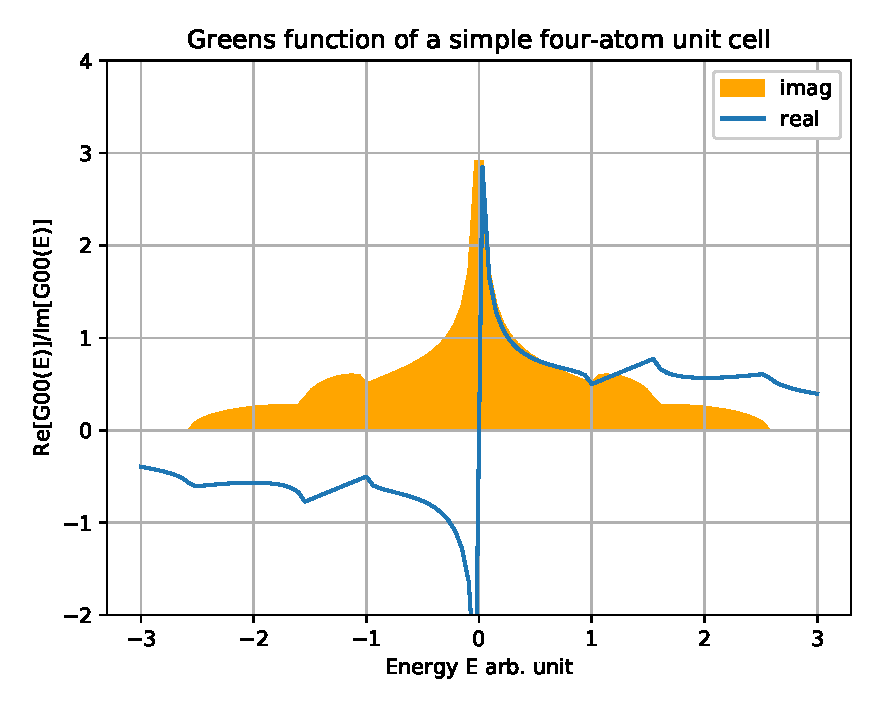
\includegraphics[width = 0.5\textwidth]{Figures/imrealplot.eps}
    \caption{A plot showing the real and imaginary part of the first cell Green's function resulting from the recursion routine on the simple system. Note that the yellow imaginary part is the representation of the density of states.}
    \label{imrealplot}
\end{figure}
